\documentclass[twoside]{book}

% Packages required by doxygen
\usepackage{fixltx2e}
\usepackage{calc}
\usepackage{doxygen}
\usepackage[export]{adjustbox} % also loads graphicx
\usepackage{graphicx}
\usepackage[utf8]{inputenc}
\usepackage{makeidx}
\usepackage{multicol}
\usepackage{multirow}
\PassOptionsToPackage{warn}{textcomp}
\usepackage{textcomp}
\usepackage[nointegrals]{wasysym}
\usepackage[table]{xcolor}

% Font selection
\usepackage[T1]{fontenc}
\usepackage[scaled=.90]{helvet}
\usepackage{courier}
\usepackage{amssymb}
\usepackage{sectsty}
\renewcommand{\familydefault}{\sfdefault}
\allsectionsfont{%
  \fontseries{bc}\selectfont%
  \color{darkgray}%
}
\renewcommand{\DoxyLabelFont}{%
  \fontseries{bc}\selectfont%
  \color{darkgray}%
}
\newcommand{\+}{\discretionary{\mbox{\scriptsize$\hookleftarrow$}}{}{}}

% Page & text layout
\usepackage{geometry}
\geometry{%
  a4paper,%
  top=2.5cm,%
  bottom=2.5cm,%
  left=2.5cm,%
  right=2.5cm%
}
\tolerance=750
\hfuzz=15pt
\hbadness=750
\setlength{\emergencystretch}{15pt}
\setlength{\parindent}{0cm}
\setlength{\parskip}{3ex plus 2ex minus 2ex}
\makeatletter
\renewcommand{\paragraph}{%
  \@startsection{paragraph}{4}{0ex}{-1.0ex}{1.0ex}{%
    \normalfont\normalsize\bfseries\SS@parafont%
  }%
}
\renewcommand{\subparagraph}{%
  \@startsection{subparagraph}{5}{0ex}{-1.0ex}{1.0ex}{%
    \normalfont\normalsize\bfseries\SS@subparafont%
  }%
}
\makeatother

% Headers & footers
\usepackage{fancyhdr}
\pagestyle{fancyplain}
\fancyhead[LE]{\fancyplain{}{\bfseries\thepage}}
\fancyhead[CE]{\fancyplain{}{}}
\fancyhead[RE]{\fancyplain{}{\bfseries\leftmark}}
\fancyhead[LO]{\fancyplain{}{\bfseries\rightmark}}
\fancyhead[CO]{\fancyplain{}{}}
\fancyhead[RO]{\fancyplain{}{\bfseries\thepage}}
\fancyfoot[LE]{\fancyplain{}{}}
\fancyfoot[CE]{\fancyplain{}{}}
\fancyfoot[RE]{\fancyplain{}{\bfseries\scriptsize Generated by Doxygen }}
\fancyfoot[LO]{\fancyplain{}{\bfseries\scriptsize Generated by Doxygen }}
\fancyfoot[CO]{\fancyplain{}{}}
\fancyfoot[RO]{\fancyplain{}{}}
\renewcommand{\footrulewidth}{0.4pt}
\renewcommand{\chaptermark}[1]{%
  \markboth{#1}{}%
}
\renewcommand{\sectionmark}[1]{%
  \markright{\thesection\ #1}%
}

% Indices & bibliography
\usepackage{natbib}
\usepackage[titles]{tocloft}
\setcounter{tocdepth}{3}
\setcounter{secnumdepth}{5}
\makeindex

% Hyperlinks (required, but should be loaded last)
\usepackage{ifpdf}
\ifpdf
  \usepackage[pdftex,pagebackref=true]{hyperref}
\else
  \usepackage[ps2pdf,pagebackref=true]{hyperref}
\fi
\hypersetup{%
  colorlinks=true,%
  linkcolor=blue,%
  citecolor=blue,%
  unicode%
}

% Custom commands
\newcommand{\clearemptydoublepage}{%
  \newpage{\pagestyle{empty}\cleardoublepage}%
}

\usepackage{caption}
\captionsetup{labelsep=space,justification=centering,font={bf},singlelinecheck=off,skip=4pt,position=top}

%===== C O N T E N T S =====

\begin{document}

% Titlepage & ToC
\hypersetup{pageanchor=false,
             bookmarksnumbered=true,
             pdfencoding=unicode
            }
\pagenumbering{alph}
\begin{titlepage}
\vspace*{7cm}
\begin{center}%
{\Large Water\+Minimizer \\[1ex]\large 1.\+0 }\\
\vspace*{1cm}
{\large Generated by Doxygen 1.8.13}\\
\end{center}
\end{titlepage}
\clearemptydoublepage
\pagenumbering{roman}
\tableofcontents
\clearemptydoublepage
\pagenumbering{arabic}
\hypersetup{pageanchor=true}

%--- Begin generated contents ---
\chapter{File Index}
\section{File List}
Here is a list of all files with brief descriptions\+:\begin{DoxyCompactList}
\item\contentsline{section}{\hyperlink{water__optimize_8f90}{water\+\_\+optimize.\+f90} }{\pageref{water__optimize_8f90}}{}
\end{DoxyCompactList}

\chapter{File Documentation}
\hypertarget{water__optimize_8f90}{}\section{water\+\_\+optimize.\+f90 File Reference}
\label{water__optimize_8f90}\index{water\+\_\+optimize.\+f90@{water\+\_\+optimize.\+f90}}
\subsection*{Functions/\+Subroutines}
\begin{DoxyCompactItemize}
\item 
program \hyperlink{water__optimize_8f90_a9bc57b8dbe7c3e1b9db72b918a1b6bab}{test}
\item 
subroutine \hyperlink{water__optimize_8f90_aa6798098feec21c5053572f5c5043c28}{readpdb} (coord, pdb)
\item 
subroutine \hyperlink{water__optimize_8f90_adad91e5491ec76f67219e4754299ceac}{minimize} (coord, force)
\item 
subroutine \hyperlink{water__optimize_8f90_a860a9ce2ec48bea8e9cd249437c3269d}{aforce} (x, force)
\item 
subroutine \hyperlink{water__optimize_8f90_ac09d0de3f934f24e9272c2f52a8eb350}{double\+\_\+cross\+\_\+product} (v1, v2, cp)
\item 
subroutine \hyperlink{water__optimize_8f90_a04c9baacf7d82c67687c579db9ec3446}{cross\+\_\+product\+\_\+3d} (v1, v2, v3)
\item 
subroutine \hyperlink{water__optimize_8f90_a1c61ecd9ef781071e23a3290f6371c4d}{bforce} (coord, force)
\end{DoxyCompactItemize}


\subsection{Function/\+Subroutine Documentation}
\mbox{\Hypertarget{water__optimize_8f90_a860a9ce2ec48bea8e9cd249437c3269d}\label{water__optimize_8f90_a860a9ce2ec48bea8e9cd249437c3269d}} 
\index{water\+\_\+optimize.\+f90@{water\+\_\+optimize.\+f90}!aforce@{aforce}}
\index{aforce@{aforce}!water\+\_\+optimize.\+f90@{water\+\_\+optimize.\+f90}}
\subsubsection{\texorpdfstring{aforce()}{aforce()}}
{\footnotesize\ttfamily subroutine aforce (\begin{DoxyParamCaption}\item[{real, dimension(3,3), intent(in)}]{x,  }\item[{real, dimension(3,3), intent(inout)}]{force }\end{DoxyParamCaption})}

Here is the call graph for this function\+:
\nopagebreak
\begin{figure}[H]
\begin{center}
\leavevmode
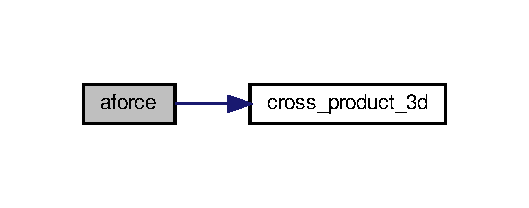
\includegraphics[width=254pt]{water__optimize_8f90_a860a9ce2ec48bea8e9cd249437c3269d_cgraph}
\end{center}
\end{figure}
Here is the caller graph for this function\+:
\nopagebreak
\begin{figure}[H]
\begin{center}
\leavevmode
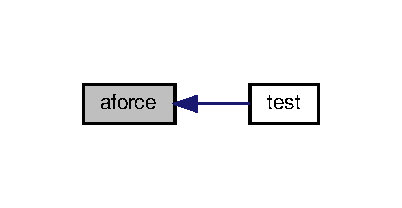
\includegraphics[width=193pt]{water__optimize_8f90_a860a9ce2ec48bea8e9cd249437c3269d_icgraph}
\end{center}
\end{figure}
\mbox{\Hypertarget{water__optimize_8f90_a1c61ecd9ef781071e23a3290f6371c4d}\label{water__optimize_8f90_a1c61ecd9ef781071e23a3290f6371c4d}} 
\index{water\+\_\+optimize.\+f90@{water\+\_\+optimize.\+f90}!bforce@{bforce}}
\index{bforce@{bforce}!water\+\_\+optimize.\+f90@{water\+\_\+optimize.\+f90}}
\subsubsection{\texorpdfstring{bforce()}{bforce()}}
{\footnotesize\ttfamily subroutine bforce (\begin{DoxyParamCaption}\item[{real, dimension(3,3), intent(inout)}]{coord,  }\item[{real, dimension(3,3), intent(inout)}]{force }\end{DoxyParamCaption})}

Here is the caller graph for this function\+:
\nopagebreak
\begin{figure}[H]
\begin{center}
\leavevmode
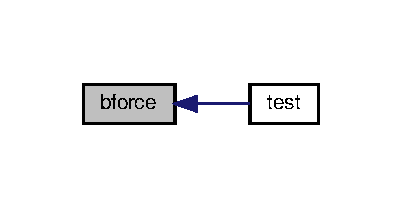
\includegraphics[width=193pt]{water__optimize_8f90_a1c61ecd9ef781071e23a3290f6371c4d_icgraph}
\end{center}
\end{figure}
\mbox{\Hypertarget{water__optimize_8f90_a04c9baacf7d82c67687c579db9ec3446}\label{water__optimize_8f90_a04c9baacf7d82c67687c579db9ec3446}} 
\index{water\+\_\+optimize.\+f90@{water\+\_\+optimize.\+f90}!cross\+\_\+product\+\_\+3d@{cross\+\_\+product\+\_\+3d}}
\index{cross\+\_\+product\+\_\+3d@{cross\+\_\+product\+\_\+3d}!water\+\_\+optimize.\+f90@{water\+\_\+optimize.\+f90}}
\subsubsection{\texorpdfstring{cross\+\_\+product\+\_\+3d()}{cross\_product\_3d()}}
{\footnotesize\ttfamily subroutine cross\+\_\+product\+\_\+3d (\begin{DoxyParamCaption}\item[{real, dimension(3), intent(in)}]{v1,  }\item[{real, dimension(3), intent(in)}]{v2,  }\item[{real, dimension(3), intent(out)}]{v3 }\end{DoxyParamCaption})}

Here is the caller graph for this function\+:
\nopagebreak
\begin{figure}[H]
\begin{center}
\leavevmode
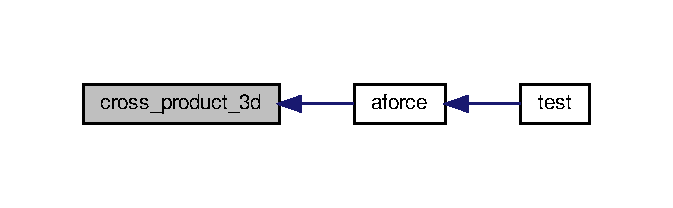
\includegraphics[width=323pt]{water__optimize_8f90_a04c9baacf7d82c67687c579db9ec3446_icgraph}
\end{center}
\end{figure}
\mbox{\Hypertarget{water__optimize_8f90_ac09d0de3f934f24e9272c2f52a8eb350}\label{water__optimize_8f90_ac09d0de3f934f24e9272c2f52a8eb350}} 
\index{water\+\_\+optimize.\+f90@{water\+\_\+optimize.\+f90}!double\+\_\+cross\+\_\+product@{double\+\_\+cross\+\_\+product}}
\index{double\+\_\+cross\+\_\+product@{double\+\_\+cross\+\_\+product}!water\+\_\+optimize.\+f90@{water\+\_\+optimize.\+f90}}
\subsubsection{\texorpdfstring{double\+\_\+cross\+\_\+product()}{double\_cross\_product()}}
{\footnotesize\ttfamily subroutine double\+\_\+cross\+\_\+product (\begin{DoxyParamCaption}\item[{real, dimension(3), intent(in)}]{v1,  }\item[{real, dimension(3), intent(in)}]{v2,  }\item[{real, dimension(3), intent(out)}]{cp }\end{DoxyParamCaption})}

\mbox{\Hypertarget{water__optimize_8f90_adad91e5491ec76f67219e4754299ceac}\label{water__optimize_8f90_adad91e5491ec76f67219e4754299ceac}} 
\index{water\+\_\+optimize.\+f90@{water\+\_\+optimize.\+f90}!minimize@{minimize}}
\index{minimize@{minimize}!water\+\_\+optimize.\+f90@{water\+\_\+optimize.\+f90}}
\subsubsection{\texorpdfstring{minimize()}{minimize()}}
{\footnotesize\ttfamily subroutine minimize (\begin{DoxyParamCaption}\item[{real, dimension(3,3), intent(inout)}]{coord,  }\item[{real, dimension(3,3), intent(in)}]{force }\end{DoxyParamCaption})}

Here is the caller graph for this function\+:
\nopagebreak
\begin{figure}[H]
\begin{center}
\leavevmode
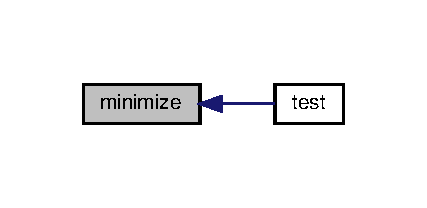
\includegraphics[width=205pt]{water__optimize_8f90_adad91e5491ec76f67219e4754299ceac_icgraph}
\end{center}
\end{figure}
\mbox{\Hypertarget{water__optimize_8f90_aa6798098feec21c5053572f5c5043c28}\label{water__optimize_8f90_aa6798098feec21c5053572f5c5043c28}} 
\index{water\+\_\+optimize.\+f90@{water\+\_\+optimize.\+f90}!readpdb@{readpdb}}
\index{readpdb@{readpdb}!water\+\_\+optimize.\+f90@{water\+\_\+optimize.\+f90}}
\subsubsection{\texorpdfstring{readpdb()}{readpdb()}}
{\footnotesize\ttfamily subroutine readpdb (\begin{DoxyParamCaption}\item[{real, dimension(3,3)}]{coord,  }\item[{character(len=30), dimension(3)}]{pdb }\end{DoxyParamCaption})}

Here is the caller graph for this function\+:
\nopagebreak
\begin{figure}[H]
\begin{center}
\leavevmode
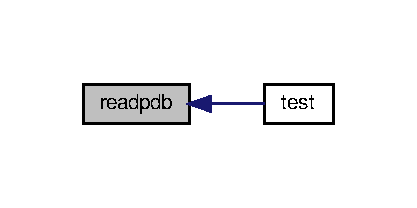
\includegraphics[width=200pt]{water__optimize_8f90_aa6798098feec21c5053572f5c5043c28_icgraph}
\end{center}
\end{figure}
\mbox{\Hypertarget{water__optimize_8f90_a9bc57b8dbe7c3e1b9db72b918a1b6bab}\label{water__optimize_8f90_a9bc57b8dbe7c3e1b9db72b918a1b6bab}} 
\index{water\+\_\+optimize.\+f90@{water\+\_\+optimize.\+f90}!test@{test}}
\index{test@{test}!water\+\_\+optimize.\+f90@{water\+\_\+optimize.\+f90}}
\subsubsection{\texorpdfstring{test()}{test()}}
{\footnotesize\ttfamily program test (\begin{DoxyParamCaption}{ }\end{DoxyParamCaption})}

Here is the call graph for this function\+:
\nopagebreak
\begin{figure}[H]
\begin{center}
\leavevmode
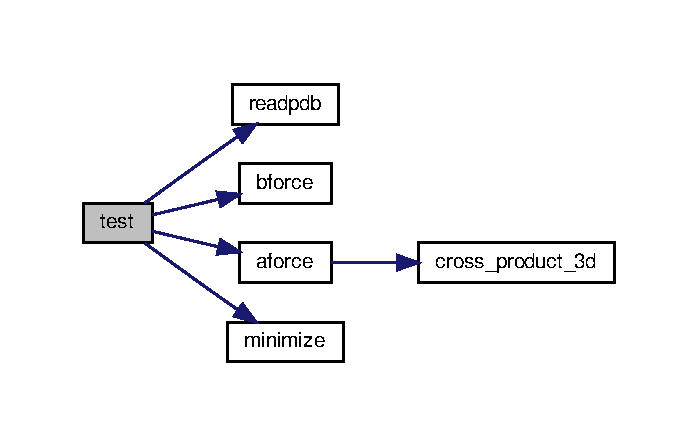
\includegraphics[width=335pt]{water__optimize_8f90_a9bc57b8dbe7c3e1b9db72b918a1b6bab_cgraph}
\end{center}
\end{figure}

%--- End generated contents ---

% Index
\backmatter
\newpage
\phantomsection
\clearemptydoublepage
\addcontentsline{toc}{chapter}{Index}
\printindex

\end{document}
